\newpage
\section{SIR-Modell für Deutschland}\label{sec:Resultate-SIR}
Wie in \autoref{sec:Vorgehensweise:SIR} beschrieben, sind in den drei Graphen in \autoref{fig:SIR_Deutschland} die drei Kennzahlen des SIR-Modells für Deutschland dargestellt.

Von den 3~748~038 gemeldeten Fällen weisen 46~033 Meldungen (1,2\%) nachfolgend beschriebenen Inkonsistenzen auf. Dies entspricht fast der maximalen Zahl der Menschen in Kategorie \glqq{}Infectious\grqq{} von circa 60~000.

In 37~757 Fällen liegt das Meldedatum vor dem Referenzdatum, das heißt die Person ist nach der hier verwendeten Interpretation genesen, beziehungsweise gestorben, bevor sie sich angesteckt hat. Bei diesen Meldungen wird das Meldedatum auf das Referenzdatum gesetzt.
In 8276 Fällen liegt das Referenzdatum mehr als 30~Tage vor dem Meldedatum, die Person ist also mehr als 30~Tage krank, was laut RKI sehr unwahrscheinlich ist.\autocite{RKI_Bulletin} Auch in diesen Fällen wird das Meldedatum auf das Referenzdatum gesetzt.

1409 Fälle wurden vor dem 01. März 2020 an das RKI gemeldet. Teilweise handelt es sich um authentische Meldungen, teilweise um fragwürdige Meldungen. Da die Gesamtzahl jedoch unter einem Prozent liegt, werden die Fälle in \autoref{fig:SIR_Deutschland} zum 01. März 2020 hinzugerechnet.

\begin{figure}[H]
    \centering
    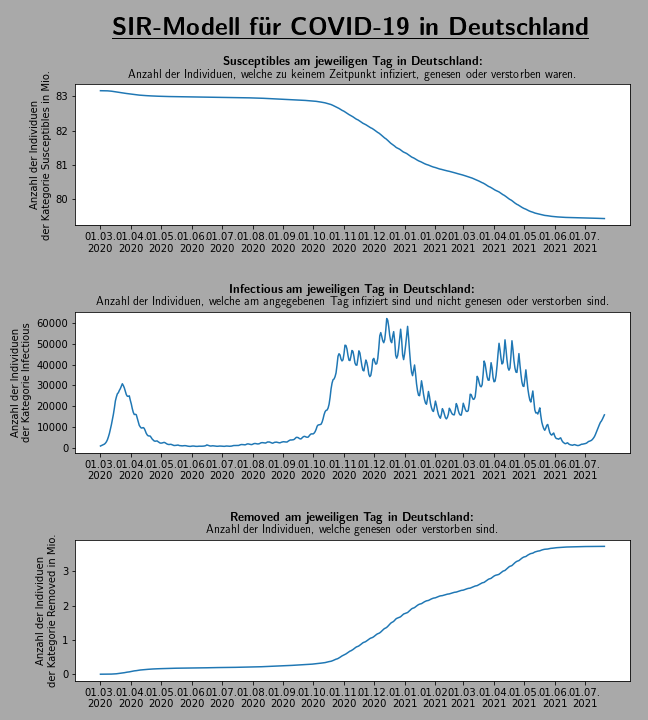
\includegraphics[width = \textwidth]{figures/Ergebnisse/SIR_Modell_Deutschland.png}
    \caption{Die drei Kennzahlen des SIR-Modells für Deutschland in drei Graphen wie sie in \autoref{sec:Grundlagen:SIR} definiert sind.}
    \label{fig:SIR_Deutschland}
\end{figure}